\normaltrue \difficilefalse \tdifficilefalse
\correctionfalse

%\UPSTIidClasse{11} % 11 sup, 12 spé
%\newcommand{\UPSTIidClasse}{12}
% ATS 2019
\exer{Le banc balafre $\star$ \label{B2:17:50}}
\setcounter{numques}{0}
\UPSTIcompetence[2]{B2-17}
\index{Compétence B2-17}
\index{Le Banc Balafre}
\index{Diagramme d'états}
\ifcorrection
\else
\textbf{Pas de corrigé pour cet exercice.}
\fi

\ifprof
\else

Pendant un essai, les actionneurs sont commandés axe par axe (c’est-à-dire par groupes
de deux actionneurs piézoélectriques) grâce à un module d’électronique de puissance
$2\times \SI{10}{kV.A}$. Ainsi, quatre modules sont installés dans l’armoire de commande. Les actionneurs
sont commandés pour générer ce que l’on appelle des « rafales » : ils produisent
les vibrations avec les caractéristiques voulues par l’opérateur, pendant une durée qui
dépend de l’objectif de l’essai en cours.

\begin{obj}
Nous allons modéliser la façon dont la commande du système
doit être programmée afin de protéger les composants vis-à-vis de problèmes de surchauffe.
\end{obj}



Afin de protéger les composants, le système de commande doit imposer des périodes de
temporisation pour favoriser le refroidissement des actionneurs et amplificateurs. Les amplificateurs
de puissance ne doivent pas être utilisés en continu pendant plus de $\text{timeout} =
\SI{10}{s}$. Le superviseur ne doit pas autoriser de temps de rafale supérieur à $t_{\text{max}} = \SI{31}{s}$. À
chaque période supérieure à timeout, il est nécessaire de temporiser le système pendant
\SI{1}{s} et pour une durée de rafale supérieure à $t_{\text{max}}$, il est nécessaire de temporiser pendant
\SI{3}{s}.
Le diagramme d’état du superviseur du banc Balafre est présenté sur la figure \ref{fig_50_01}.


\begin{figure}[H]
\centering
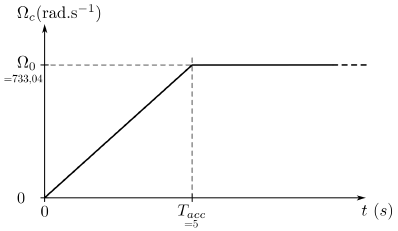
\includegraphics[width=\linewidth]{fig_50_01}
\caption{Diagramme d’état du superviseur du banc Balafre. \label{fig_50_01}}
\end{figure}
\fi

Les variables suivantes permettent de réaliser le suivi d’un processus de mesure :
\begin{itemize}
\item Démarrer est une variable booléenne. Elle devient vraie, lorsque l’opérateur a saisi
le nombre $Na$ de cycles qu’il souhaite réaliser et la durée $T_1$ de chaque cycle, et
qu’il a validé sa saisie.
\item Moteur est une variable qui vaut 1 lorsque le moteur a atteint sa vitesse de consigne
(supposée non nulle, la vitesse nulle n’étant pas une consigne d’intérêt pratique
pour le banc d’essais). Quand Moteur a atteint la valeur 1, seul le retour à l’arrêt
peut modifier l’état de cette variable en la faisant repasser à 0. On considère qu’il
faut \SI{5}{s} pour atteindre la vitesse de consigne ou revenir à l’arrêt.
\item Controle est une variable qui décrit le résultat des contrôles de la chaîne d’acquisition
:
\begin{itemize}
\item Controle=0 si les contrôles n’ont pas été effectués ;
\item Controle=1 si les contrôles sont terminés et que tout est en ordre de marche ;
\item Controle=2 si les contrôles ont détecté une anomalie.
\end{itemize}
\item Rafale est une variable qui vaut 1 si une rafale est en cours, et 0 sinon.
\end{itemize}








\question{On souhaite réaliser un cycle de rafale de huit secondes. En suivant
le diagramme d’état de la figure \ref{fig_50_01}, et en supposant que le contrôle soit réalisé en 1
seconde et conclue à ce que tout soit en ordre de marche, compléter le chronogramme.}


\begin{figure}[H]
\centering
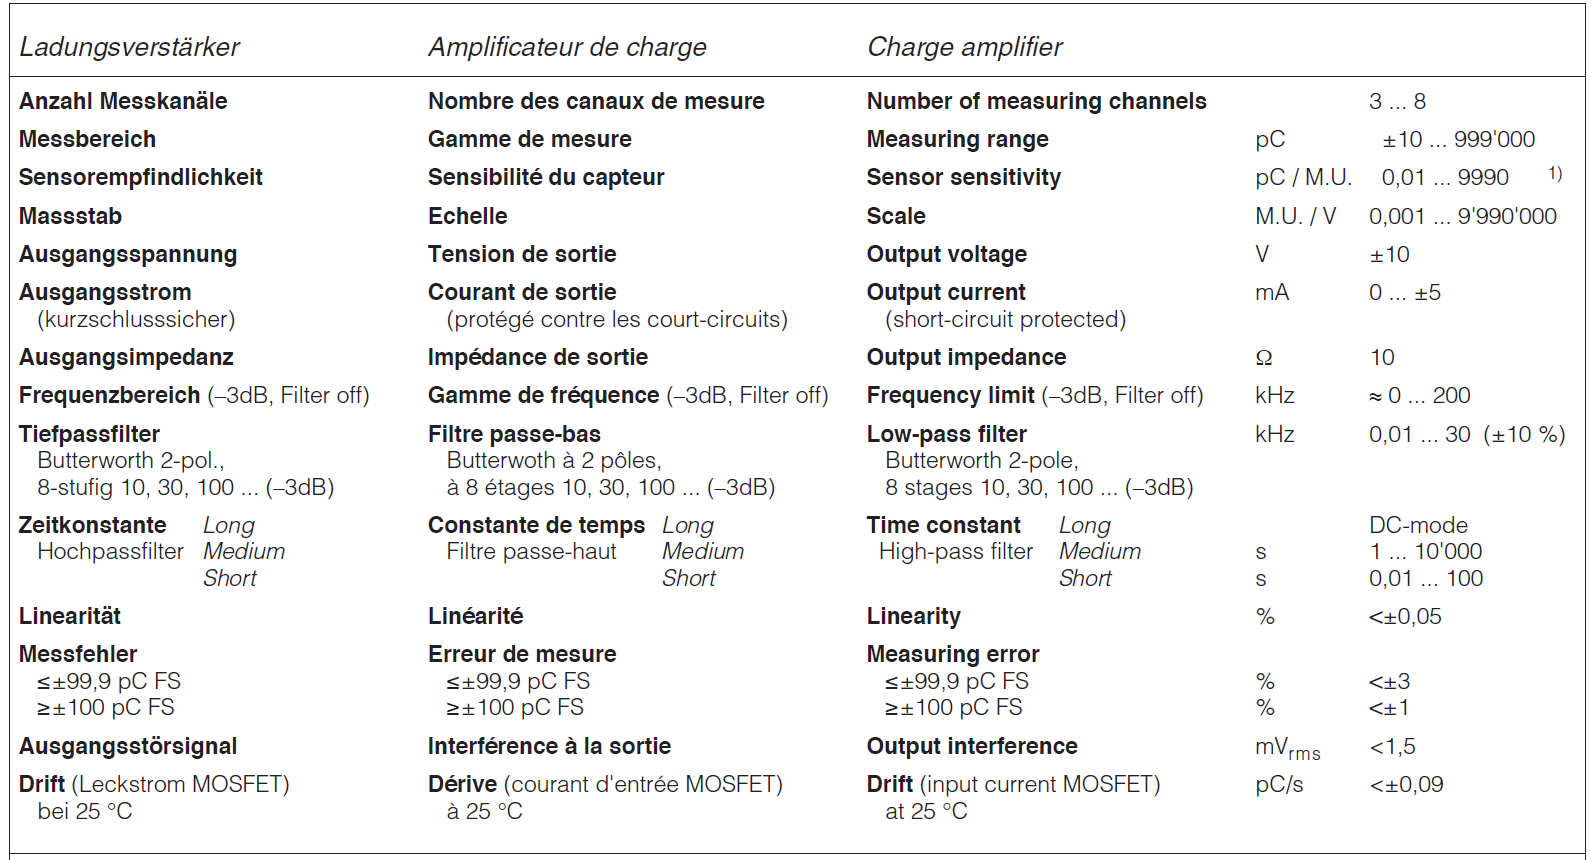
\includegraphics[width=\linewidth]{fig_50_02}
%\caption{Diagramme d’état du superviseur du banc Balafre. \label{fig_50_02}}
\end{figure}

\ifprof
\else
\fi

Pour un fonctionnement sûr de l’installation, le système doit arrêter les moteurs si les
contrôles détectent une anomalie.


\question{Modifier le diagramme d’état ci-dessous
pour prendre en compte ce cas de figure.}
\begin{figure}[H]
\centering
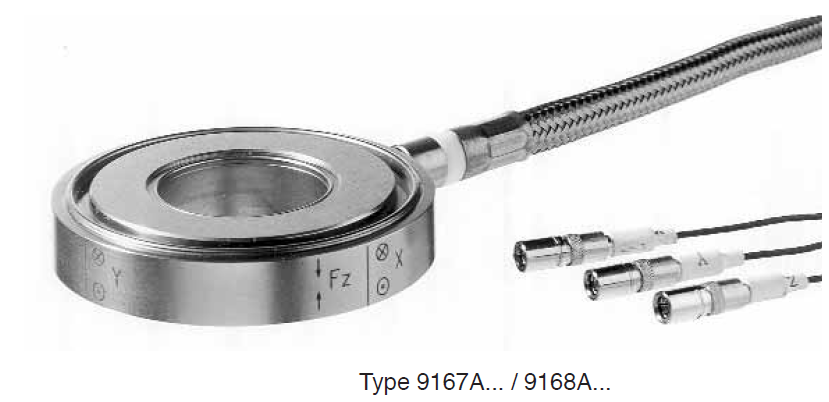
\includegraphics[width=\linewidth]{fig_50_03}
%\caption{Diagramme d’état du superviseur du banc Balafre. \label{fig_50_03}}
\end{figure}

\ifprof
\else
\fi



\ifprof
\else
\begin{flushright}
\footnotesize{Corrigé  voir \ref{B2:17:50}.}
\end{flushright}%
\fi